
\section{Assessing the Signal-to-Noise Ratio of the Gradient Estimators}
\label{sec:snr}
Because it is not feasible to analytically optimize these \glspl{ELBO} in complex models,  the effectiveness of any particular choice of \gls{ELBO} is linked
to our ability to numerically solve the resulting optimization problem. This motivates us to examine 
the effect $K$ has on the variance and magnitude of the gradient estimates of \gls{IWAE} for the two networks. More generally, we study \gls{IWAE} gradient estimators constructed as the average of $M$ estimates, each built from $K$ independent particles. We present a result characterizing the asymptotic signal-to-noise ratio in $M$ and $K$. For the standard case of $M=1$, our result shows that the signal-to-noise ratio of the reparameterization gradients of the inference network for the \gls{IWAE} decreases with rate $O(1/\sqrt{K})$.

As estimating the $\ELBO$ requires a Monte Carlo estimation of an expectation over $z$, 
we have two sample sizes to tune for the estimate:
the number of samples $M$ used for Monte Carlo estimation of the \gls{ELBO} and the number of importance samples $K$ used
in the bound construction.  Here $M$ does not change the true value of
$\nabla_{\theta, \phi} \ELBO$, only our variance in estimating
it, while changing $K$ changes the \gls{ELBO} itself, with larger $K$ leading to tighter 
bounds~\citep{Burda2016importance}.  Presuming that reparameterization
is possible, we can express our gradient estimate in the general form
\begin{align}
\label{eq:grad-est}
\Delta_{M,K} :=  &\frac{1}{M} \sum\nolimits_{m=1}^{M}
\nabla_{\theta, \phi} \log \frac{1}{K} \sum\nolimits_{k=1}^{K} w_{m,k}^{}, \\
\text{where} \, \, w_{m,k}^{} &= \frac{p_{\theta}(z_{m,k},x^{})}{q_{\phi}(z_{m,k} \given x^{})} \, \,
\text{and} \, \,z_{m,k} \sim q_{\phi}(z_{m,k} \given x^{}). \nonumber
\end{align}

Thus, for a fixed budget of $T = MK$ samples, we have a family of estimators with the cases $K=1$ and $M=1$
corresponding respectively to the \gls{VAE} and \gls{IWAE} objectives.
We will use ${\Delta}_{M,K} \left(\theta\right)$ to refer to gradient estimates with respect
to $\theta$ and ${\Delta}_{M,K} \left(\phi\right)$ for those with respect to
$\phi$. 

Variance is not always a good barometer for the effectiveness
of a gradient estimation scheme; estimators with small expected values need proportionally smaller variances to 
be estimated accurately. In the case of \gls{IWAE}, when changes in $K$ simultaneously affect both the variance and
expected value, the quality of the estimator for learning can actually \emph{worsen} as the variance decreases.
To see why, consider
the marginal likelihood estimates $\hat{Z}_{m,K}^{} =\sum_{k=1}^{K} w_{m,k}^{}$. Because these become exact (and thus independent of the proposal) as $K\to\infty$, it must be the case that 
$\lim_{K\rightarrow\infty} {\Delta}_{M,K} (\phi) = 0$. 
Thus as $K$ becomes large, the expected value of the gradient
must decrease along with its variance, such that the variance relative to the problem scaling
need not actually improve.

To investigate this formally, we introduce the signal-to-noise-ratio (\textsc{snr}),
defining it to be the absolute value of the expected estimate scaled by its standard deviation:
\begin{align}
\SNR_{M,K} (\theta) &= \left|\E \left[\Delta_{M,K} (\theta)\right]/
\sigma\left[\Delta_{M,K} (\theta)\right]\right|
\end{align}
where $\sigma [\cdot]$ denotes the standard deviation of a random variable.
The \gls{SNR} is defined separately on each dimension of the parameter vector and
similarly for $\SNR_{M,K} (\phi)$. It provides a measure of the relative accuracy of the gradient estimates. Though a high \gls{SNR}
does not always indicate a good \gls{SGA} scheme (as the target objective itself might be
poorly chosen), a low \gls{SNR} is always problematic as it indicates that
the gradient estimates are dominated by noise: if $\SNR\to0$ then the estimates
become completely random.  We are now ready to state our main
theoretical result:  
$\SNR_{M,K} (\theta) = O(\sqrt{MK})$ and
$\SNR_{M,K} (\phi) = O(\sqrt{M/K})$.

\begin{restatable}{theorem}{snrproof}
	\label{the:snr}
Assume that when $M=K=1$, the expected gradients; the variances of the gradients; and the 
first four moments of  $w_{1,1}$, $\nabla_{\theta} w_{1,1}$, and 
$\nabla_{\phi} w_{1,1}$ are all finite and the variances are
also non-zero.
Then the signal-to-noise ratios of the gradient estimates converge at the following rates
\begin{align}
&\SNR_{M,K} (\theta) = 
	\label{eq:snr_theta} \\
&\sqrt{M}\left|\frac{ \sqrt{K} \; 
	\nabla_{\theta} Z -\frac{1}{2Z\sqrt{K}}\nabla_{\theta} \left(\frac{\textnormal{Var} \left[w_{1,1}\right]}{Z^2}\right)+ O\left(\frac{1}{K^{3/2}}\right) }
{\sqrt{\E \left[w_{1,1}^2\left(\nabla_{\theta} \log w_{1,1}-\nabla_{\theta} \log Z\right)^2\right]} + O\left(\frac{1}{K}\right)}\right| \nonumber \\
\label{eq:snr_phi}
& \SNR_{M,K} (\phi) =\sqrt{M} \left|\frac{
	\nabla_{\phi} \textnormal{Var} \left[w_{1,1}\right] + O\left(\frac{1}{K}\right) }
{2 Z\sqrt{K} \; \sigma\left[\nabla_{\phi} w_{1,1}\right] +O\left(\frac{1}{\sqrt{K}}\right)}\right|
\end{align}
where $Z := p_{\theta}(x)$ is the true marginal likelihood.
\end{restatable}
\begin{proof}
    We give an intuitive demonstration
	of the result here and provide a formal proof in Appendix~\ref{sec:proof}.
	The effect of $M$ on the \gls{SNR} follows from
	using the law of large
	numbers on the random variable $\nabla_{\theta, \phi} \log \hat{Z}_{m,K}$.  Namely, the 
	overall expectation is independent of $M$ and
	the variance reduces at a rate $O(1/M)$.  
	The effect of $K$ is more complicated but
	is perhaps most easily seen by noting that~\cite{Burda2016importance}
	\begin{align*}
	\nabla_{\theta, \phi} \log \hat{Z}_{m,K}
	= \sum_{k=1}^{K} \frac{w_{m,k}^{}}{\sum_{\ell=1}^{K} w_{m,k}^{}} 
	\nabla_{\theta, \phi} \log \left(w_{m,k}^{}\right),
	\end{align*}
	such that $\nabla_{\theta, \phi} \log \hat{Z}_{m,K}$ can be interpreted as a self-normalized importance sampling
	estimate.  We can, therefore, invoke the known result (see e.g.~\citet{Hesterberg1988advances}) 
	that the bias of a self-normalized
	importance sampler converges at a rate $O(1/K)$ and the standard deviation at
	a rate $O(1/\sqrt{K})$.  We thus see that the \gls{SNR} converges at a rate $O((1/K)/(1/\sqrt{K}))
	=O(1/\sqrt{K})$ if the asymptotic gradient is $0$ and $O((1)/(1/\sqrt{K}))=O(\sqrt{K})$
	otherwise, giving the convergence rates in the $\phi$ and $\theta$ cases respectively.
	\vspace{-8pt}
\end{proof}

The implication of these rates is that increasing $M$ is monotonically beneficial to
the \gls{SNR} for both $\theta$ and $\phi$, but that increasing $K$ is beneficial to the
former and detrimental to the latter.  We emphasize that this means the \gls{SNR} for the \gls{IWAE} inference network
gets worse as we increase $K$: this is not just an opportunity cost
from the fact that we could have increased $M$ instead, increasing the total number of samples
used in the estimator actually worsens the \gls{SNR}!

\subsection{Asymptotic Direction}
\label{sec:dir}

Even though the magnitude of the inference
network gradient estimates diminish with increasing $K$, the \emph{direction}
of the true gradient still converges to a fixed vector.
Namely, we have as an intermediary result from deriving~\eqref{eq:snr_phi}
that
\begin{align}
\label{eq:expt}
\hspace{-3pt}
\E \left[\Delta_{M,K} (\phi)\right] = -\frac{\nabla_{\phi} \text{Var}\left[w_{1,1}\right]}{2K Z^2} 
+O\left(\frac{1}{K^2}\right),
\end{align}
and we see that expected gradient points in the direction of
$-\nabla_{\phi} \text{Var}\left[w_{1,1}\right]$ as $K \to \infty$.  
This direction is rather interesting: it implies that as $K\to\infty$, the optimal $\phi$
is that which minimizes the variance of the weights.  This is well known to be 
the optimal importance sampling
distribution in terms of estimating the marginal likelihood~\citep{Mcbook}.
Given that the role of the inference network during training is to estimate the
marginal likelihood, this is thus arguably exactly what we want to optimize for.  
As such, this result, which complements those
of~\cite{Cremer2017reinterpreting}, suggests that increasing 
$K$ provides a preferable target in terms of the direction of the
true inference network gradients.  We thus see that there is a trade-off with the fact that increasing $K$ also diminishes
the \gls{SNR}, reducing the estimates to pure noise if $K$ is
set too high.   In the absence of other factors, there may thus be a ``sweet-spot'' for 
setting $K$.

\begin{figure*}[t]
	\centering
	\begin{subfigure}[b]{0.4\textwidth}
		\centering
		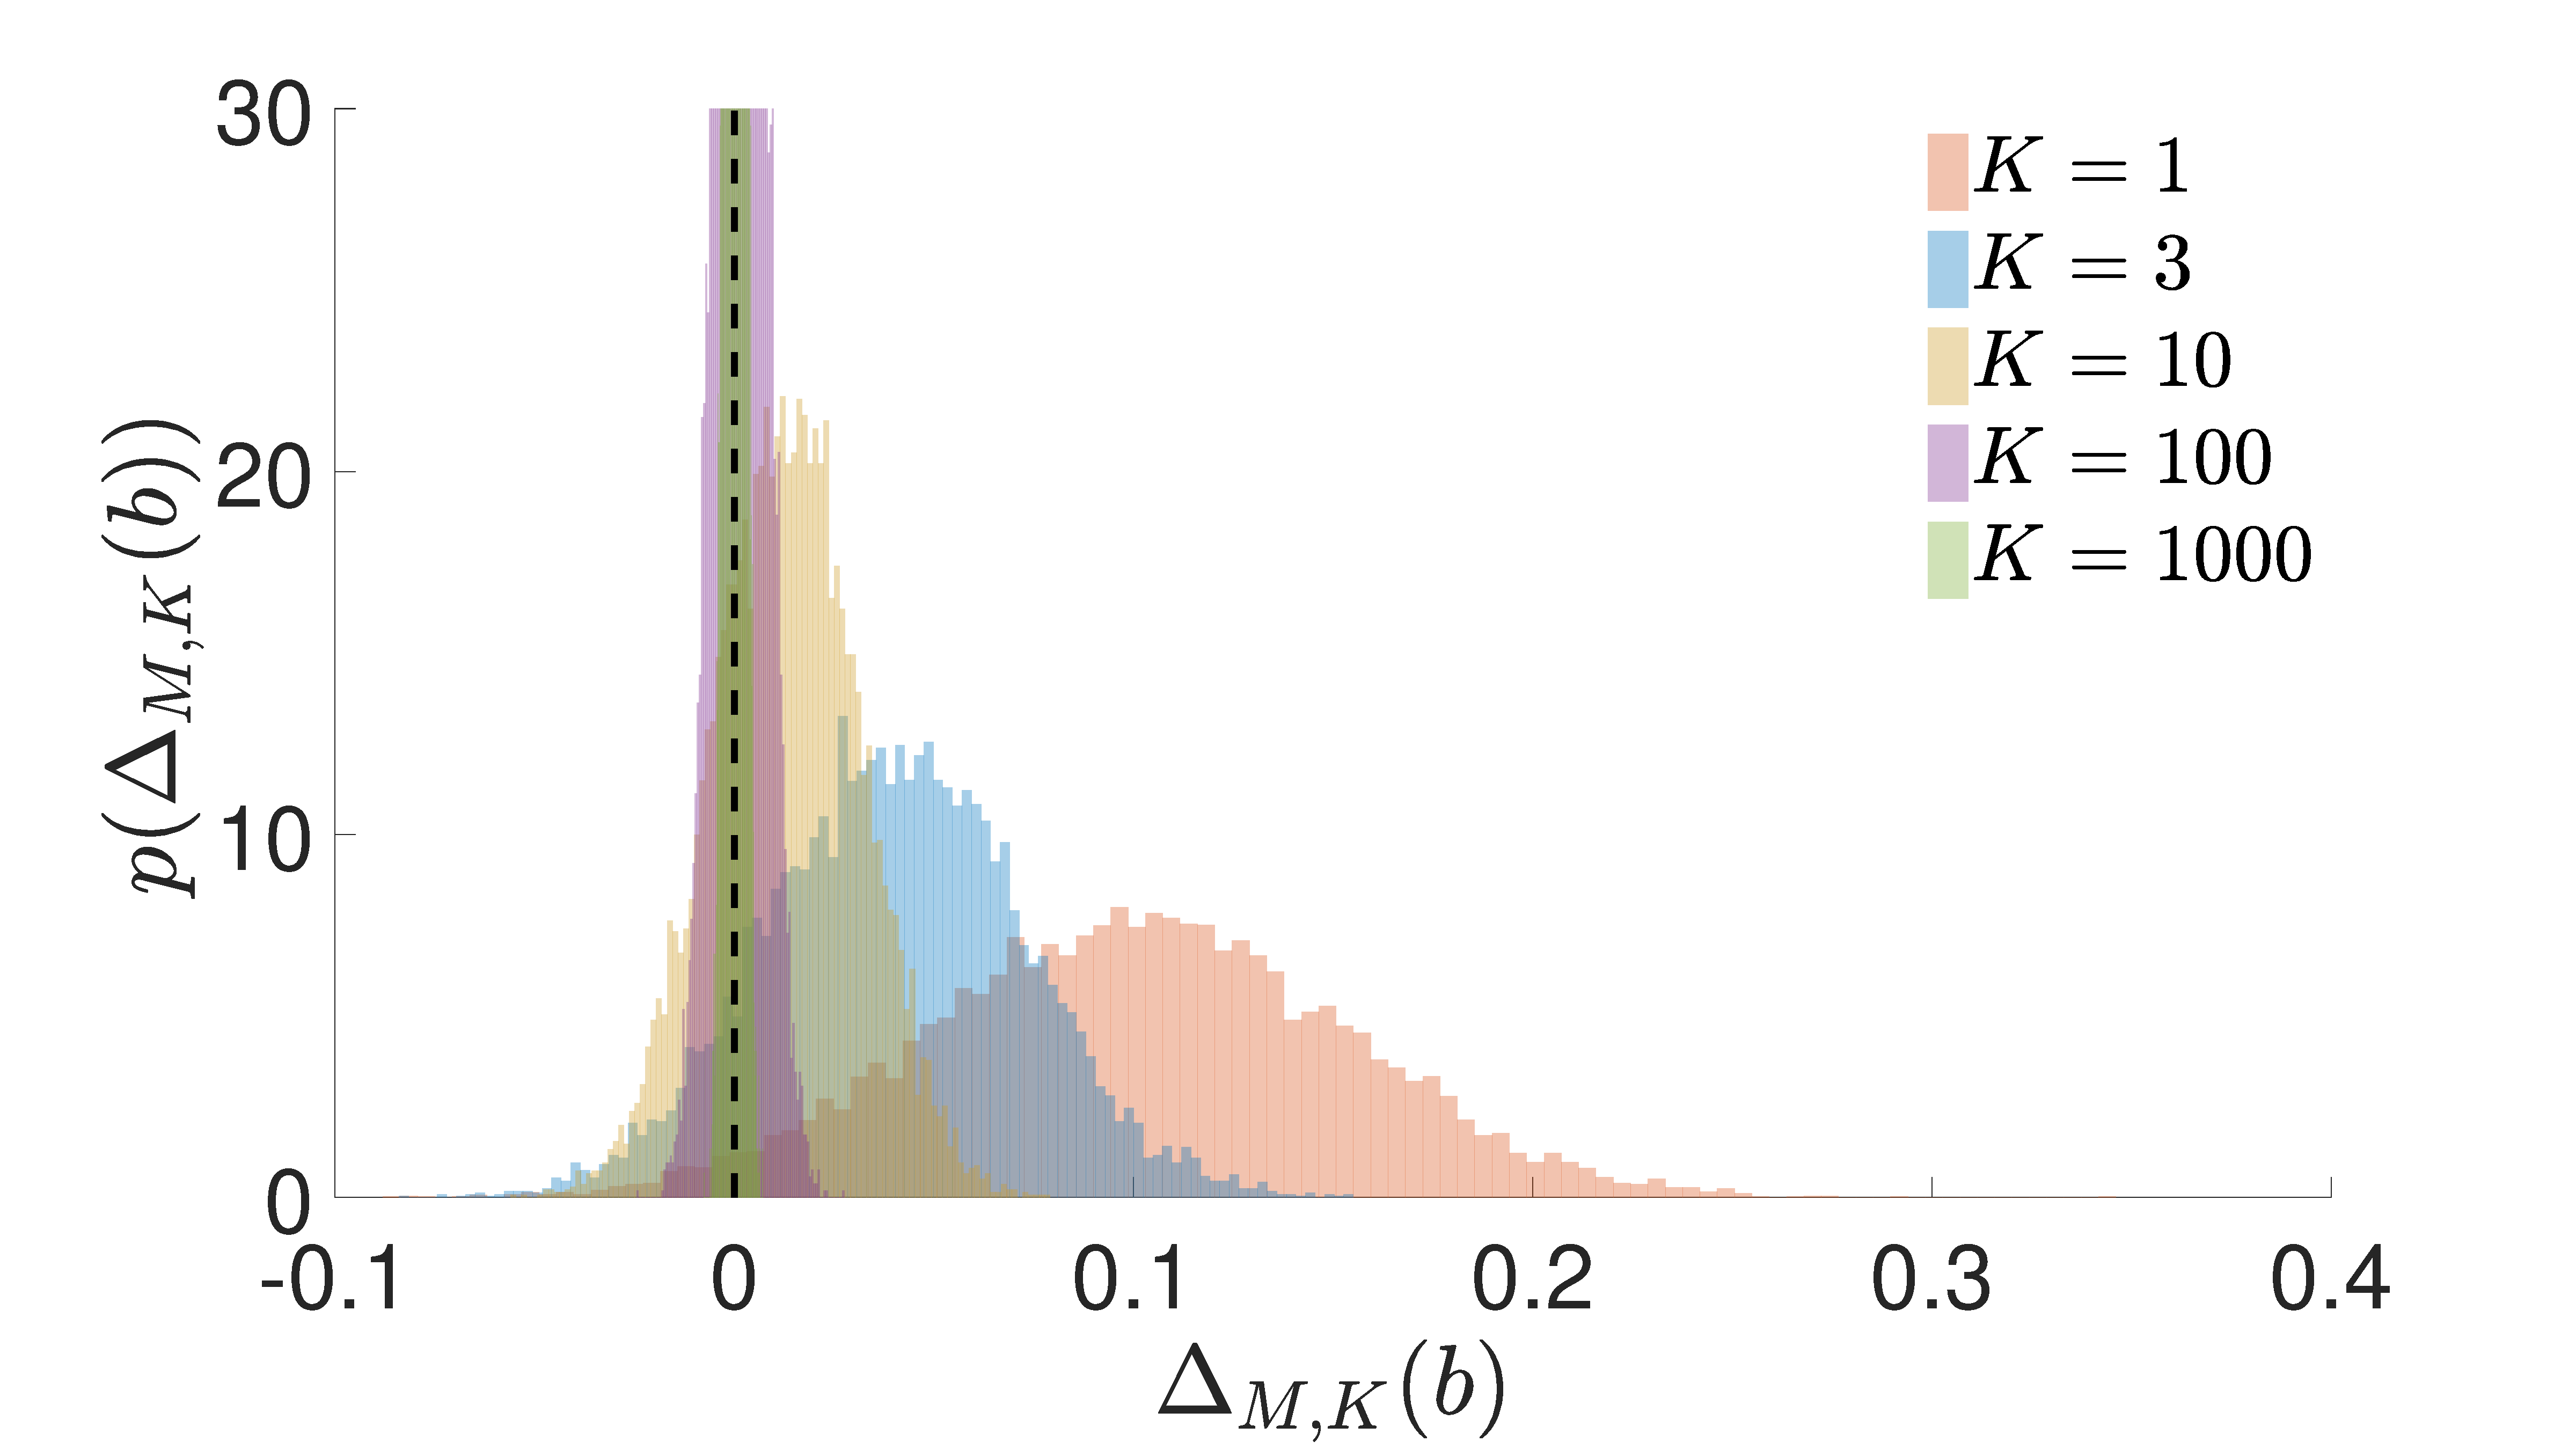
\includegraphics[width=\textwidth]{figures/tighter_bounds/b_hist_IWAE} %
		\caption{ \gls{IWAE} inference network gradient estimates \label{fig:snr/b_hist_iwae}}
	\end{subfigure} ~~~~~~~~~~~~~
	\begin{subfigure}[b]{0.4\textwidth}
		\centering
		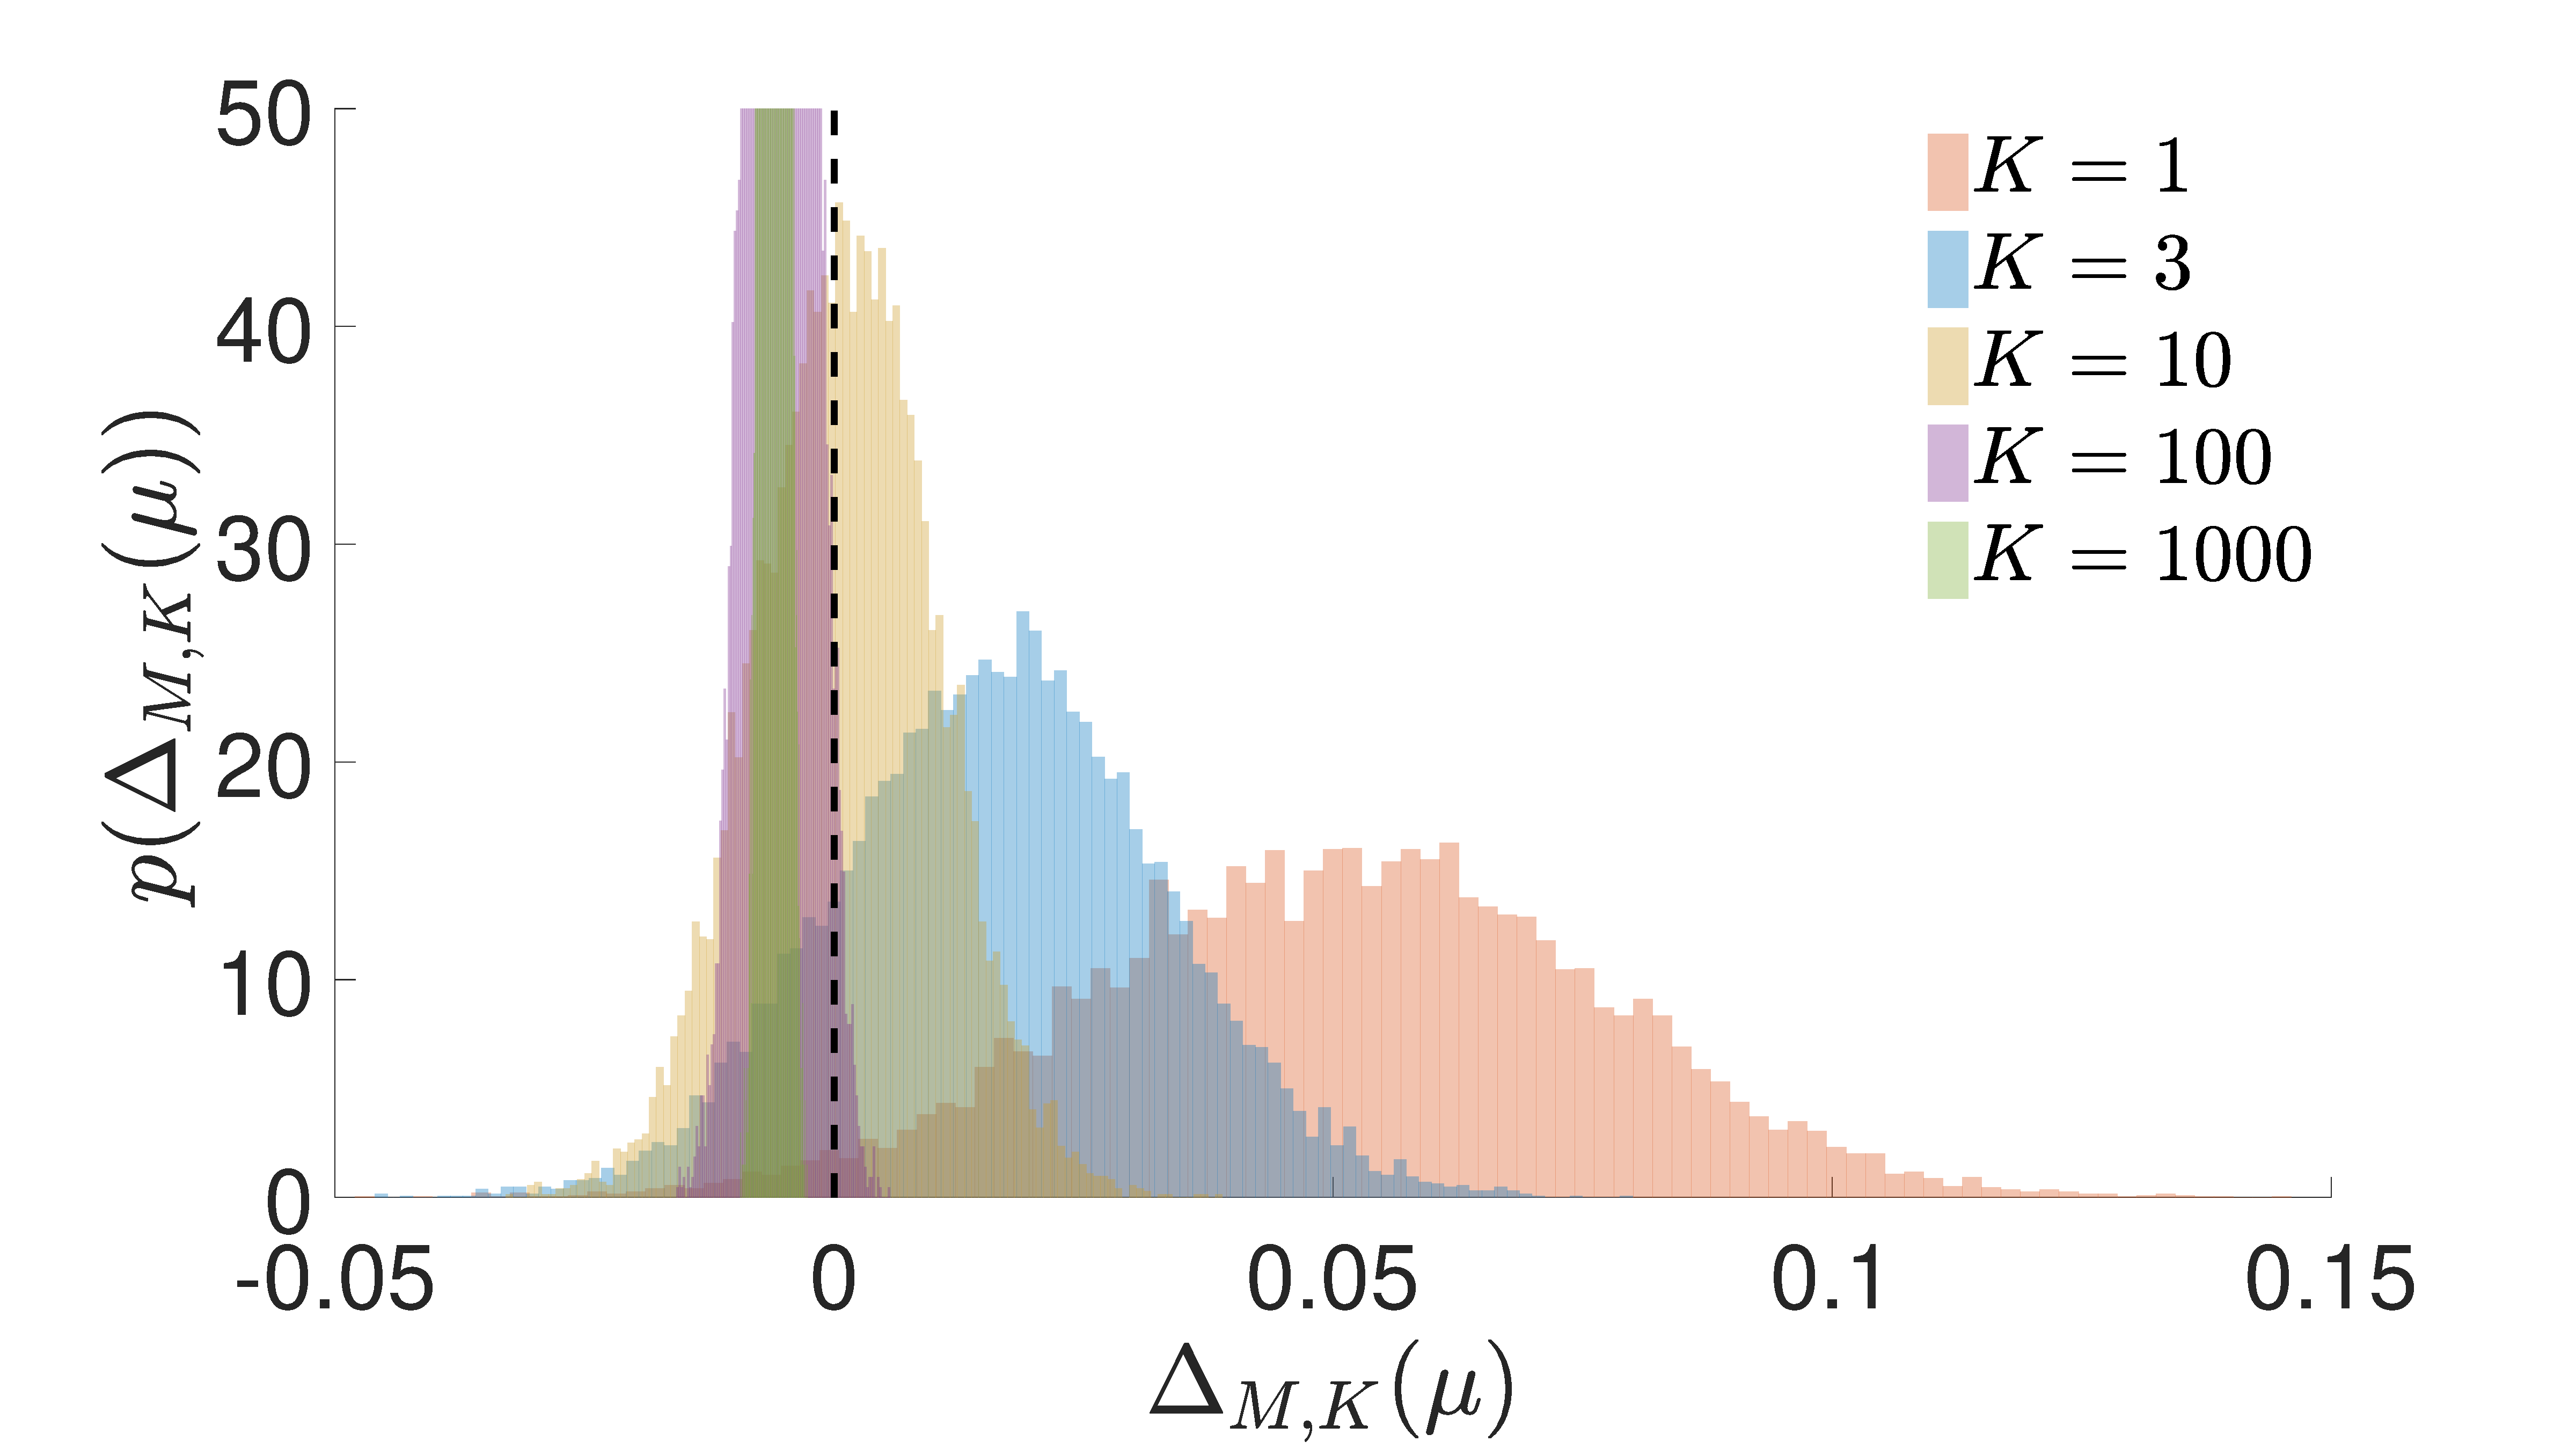
\includegraphics[width=\textwidth]{figures/tighter_bounds/mu_hist_IWAE} %
		\caption{ \gls{IWAE} generative network gradient estimates \label{fig:snr/mu_hist_iwae}}
	\end{subfigure}\vspace{-6pt}
	\caption{Histograms of gradient estimates $\Delta_{M,K}$ for the generative network and 
		the inference network using the \gls{IWAE} ($M=1$)
		objective with different values of $K$.
			\vspace{-14pt}
		\label{fig:snr/hists}}
\end{figure*}

\subsection{Multiple Data Points}
\label{sec:multi}


	Typically when training deep generative models, one does not optimize a single \gls{ELBO}
	but instead its average over multiple data points, i.e.
	\begin{align}
	\label{eq:J}
	\mathcal J(\theta, \phi) &:= 
	\frac{1}{N} \sum\nolimits_{n = 1}^N \ELBO_{\text{IS}} (\theta, \phi, x^{(n)}).
	\end{align}
	Our results extend to this setting because the $z$ are drawn independently for each $x^{(n)}$, so
	\begin{align}
	\hspace{-4pt}\E\left[\frac{1}{N} \sum\nolimits_{n=1}^{N} \Delta_{M,K}^{(n)}\right]\hspace{-2pt} &=\hspace{-2pt}\frac{1}{N}\sum\nolimits_{n=1}^{N}
	\E\left[\Delta_{M,K}^{(n)}\right], \displaybreak[0] \\
	\hspace{-4pt}\text{Var}\left[\frac{1}{N} \sum\nolimits_{n=1}^{N} \Delta_{M,K}^{(n)}\right]\hspace{-2pt} &=\hspace{-2pt}\frac{1}{N^2}\sum\nolimits_{n=1}^{N}
	\text{Var}\left[\Delta_{M,K}^{(n)}\right]\hspace{-2pt}.
	\end{align}
	We thus also see that if we are using mini-batches such that $N$ is a chosen parameter and the $x^{(n)}$ are
	drawn from the empirical data distribution, then 
	the \glspl{SNR} of $\bar{\Delta}_{N,M,K} := \frac{1}{N} \sum_{n=1}^{N} \Delta_{M,K}^{(n)}$ scales as $\sqrt{N}$, i.e.
$\SNR_{N,M,K} (\theta) = O(\sqrt{NMK})$ and $\SNR_{N,M,K} (\phi) 
= O(\sqrt{NM/K})$.  Therefore increasing $N$ has the same ubiquitous benefit as increasing $M$.
In the rest of the paper, we will implicitly be considering the \glspl{SNR} for $\bar{\Delta}_{N,M,K}$, but
will omit the dependency on $N$ to simplify the notation.





